\begin{figure*}
%\begin{center}
\centering

\includegraphics[height=2.2cm]{figures/pinterest-pipeline.png}
\caption{Pipeline for generating interesting eBay products based on Pinterest. Pinterest is first crawled, next the pins will be ranked and filtered based on whether or not they contain useful product information, next a product keyword extractor is applied to a set of highly ranked pins, and finally the extracted keywords are used to find a relevant eBay product.}
%\end{center}
\label{fig:pinterest-pipeline}
\end{figure*}

In this section, we will discuss the issue of capturing topic
correlations when using distributional representations. It is easy to
observe manually, that even for the best topic model one can find a
pair of topics that are closely related and a pair that is much more
distant. Those interrelations between topics are 
properties that represent useful information about the model that is
possible to infer from the data, and yet
may be lost in distributional representations of words. 
This shortcoming was observed in \cite{bache:2013},
also in the context of measuring text diversity. The solution proposed
there was based on a special kind of diversity measure, Rao Diversity,
which depends on constructing a set of pairwise distances between the
topics. This is achieved by computing a topic similarity matrix based on
the topic model. We propose a more general solution to this problem,
which is also based on a topic similarity matrix. However, instead of
applying it directly to a specific diversity measure, we use it to
transform the distributional representations, thereby incorporating this
additional information into the model. The main advantage of this
approach is the flexibility in the choice of diversity measure. In
particular, \cite{bache:2013} argue that Rao Diversity has a
significant advantage in measuring document diversity compared to
Shannon entropy, which does not rely on topic distances. However, our
experiments show that topic similarity information can be successfully
incorporated into the distributional representations, so that Shannon
entropy can outperform Rao Diversity.  Next, we will explain the
intuition behind our topic-similarity transformation of the
topic-word-count matrix $\cM$. Afterwards, we will discuss the
construction of the similarity matrix $\cS$.

One possible interpretation of pairwise topic similarities is as a
matrix of conditional probabilities. Suppose, that $\cS_{|T|\times|T|}$ is
such a matrix, where $S_{i,j}=\pp_\cS(t_j|t_i)$ is the conditional
probability of observing topic $t_j$ in conjunction with topic $t_i$. We are not
referring to actual observations here, but rather a way of interpreting
topic similarity in the probabilistic framework. In this context, if
$\pp_\cS(t_j|t_i)$ is high, then the topics should be highly correlated with
each other. Notice that for this to be valid, the rows of matrix $\cS$
need to form proper distributions, so they need to be normalized.  
Given a distributional representation $p_w$ and the matrix
$\cS$, the vector $\tilde{p}_w=p_w \cS^T$ will be a distribution
corresponding to a random variable $X_2$ generated by a two-stage
topic sampling:
\begin{align*}
X_1&\sim p_w,\\
X_2&\sim \pp_\cS(\,\cdot\,|X_1).
\end{align*}

This transformation ensures, in particular, that topics which are
strongly correlated with each other will get similar weight in any
distributional representation. Note, that since any topic is the most
similar to itself, we should naturally expect the largest weights in
$\cS$ to appear on the diagonal. We can apply topic similarity to all
of the data directly by transforming the original word-topic-count
matrix $\cM$, obtaining $\cM_\cS=\cM\cS^T$. So, for each word-topic
assignment in the LDA model, instead of just adding $1$ to the
corresponding cell in $\cM$, we diffuse the effect of this assignment
accross the entire row for the given word.

To construct the topic similarity matrix for the LDA model, we
followed the suggestions provided in \cite{bache:2013}. In addition to
the word-topic-count matrix $\cM$, the model also provides a
document-topic-count matrix $\cN_{|D|\times|T|}$, which has for each
document a row vector describing the number of assignments for
every topic. Note, that we are referring here to the set of documents
that was used for training the topic model, which is (or at least can
be) separate from the collection of texts for which we want to measure
diversity. To estimate the similarity of topics $t_i$ and $t_j$, we
compute the cosine similarity between their corresponding columns in
$\cN$. Denoting $\cN^{(i)},\cN^{(j)}$ as those column vectors, we
write the cosine similarity as
\begin{align*}
s(i,j) = \frac{\langle\cN^{(i)}, \cN^{(j)}\rangle}{\|\cN^{(i)}\|_2\|\cN^{(j)}\|_2},
\end{align*}
where $\langle\cdot,\cdot\rangle$ represents a dot product between
two vectors. Putting the values $s(i,j)$ into a matrix, we normalize
the rows to obtain a valid matrix of conditional probabilities $\cS$.

% Let $p$ be a row vector (corresponding to some word $w$)  from the
% word-topic co-occurrence matrix $\cM_{|V|\times|T|}$ obtained from an LDA
% model. We could think of the topics as representing a basis
% $t_1,...,t_T$ in some hypothetical vector space $\cH$. In 
% this case, $p$ corresponds to a linear combination of the basis
% vectors, $\Sigma p_i t_i$. In other words, for every occurrence of
% word $w$ assigned with $i$-th topic, we add basis vector $t_i$ to the
% complete representation of $w$ in space $\cH$.
% Suppose that $\cH$ is a Hiblert space (i.e. has an inner
% product). Now, the correlation between two topics can be represented
% by the inner-product of the corresponding basis vectors (we assume those
% are unit vectors). We can consider a following alternative representation
% of a point in $\cH$:

% \bed
% Let $p\in\rr^T$ be a vector. Denote $x=\sum_{i=1}^T p_i
% t_i\in\cH$. Let $\widehat{p}\in\rr^T$ be defined so that
% \[\widehat{p}_i = \langle x,t_i\rangle.\]
% We will call $\widehat{p}$ the inner-product representation of $p$.
% \eed

% Notice, that if the considered topic basis is orthonormal, then both
% representations $p$ and $\widehat{p}$ are identical. Consider the Gram matrix
% $\Sbb=\{\langle t_i,t_j\rangle\}_{i,j}$ of all possible inner-products between
% basis vectors. If the basis is orthonormal, this is simply the identity
% matrix. Moreover, no matter which basis we choose, matrix $\Sbb$ is the
% only information we need to translate $p$ to $\widehat{p}$.

% \ber
% For any vector $p\in\rr^T$, any Hilbert space $\cH$ and a set of
% vectors $t_1,...,t_T\in\cH$, we have 
% \[\widehat{p} = p\Sbb,\]
% where $\Sbb=\{\langle t_i,t_j\rangle\}_{i,j}$ is the Gram matrix.
% \eer

% The inner-product representation allows us to incorporate the topic
% similarity information into a vector representation. Moreover, we do
% not need to directly manipulate the space $\cH$ to obtain it, except
% computing pairwise topic correlations $s_{ij}$. Once we compute matrix
% $\Sbb$, we can transform our data matrix into this new form using
% matrix multiplication $\cM'=\cM\cdot \Sbb$. Since the co-occurrence matrix
% must have nonnegative coefficients, we will require that the matrix
% $\Sbb$ also be element-wise nonnegative (which it would not
% have to be, in general). The new data matrix $\cM'$ can be interpreted
% as follows: for each original word-topic co-occurrence, we also add to
% the matrix some {\em fractional} co-occurrences of the same word with
% other topics, based on their similarity to the main topic.

% To obtain a topic similarity matrix, all we need is to write
% the topics as nonnegative vectors in a common space. When the topics
% come from an LDA model, there is two standard ways to do that: a
% distribution over words, or a distribution over documents. Following
% the analysis in \cite{bache:2013}, we used the document distributions,
% with cosine similarity as a measure of correlation. However, we use the
% topic similarities in a different way, that can not only make this
% technique applicable to any task relying on distributional word
% representations, but also outperforms the aforementioned one for
% measuring diversity.

% To illustrate the benefit of introducing topic similarities for
% measuring diversity, consider a simple case where we have a pair of words
% $S=(w_1,w_2)$, with distributional representations $P_1,P_2$, each having
% singleton support on one topic (topic similarities not
% applied). Clearly, if those topics match, we 
% have no diversity, and if they don't, we get relatively high diversity
% (assuming uniform weights of the mixture, it would be $\log 2$). Notice, that without introducing topic similarity this is
% independent of which pair of topics we are looking at. It could, for
% instance, be ``Mathematics'' and ``Physics'' (closely related), or
% ``Mathematics'' and ``Literature'' (further apart).  Applying the
% topic similarity matrix allows for this distinction to be clear and properly
% reflected in the results, because the weight from the main topic has
% to be redistributed among similar ones, making the distributions $P_1$
% and $P_2$ more comparable.

\begin{figure*}[t!]
  \centering
  \begin{subfigure}
(a)\hspace{-1mm}
    \centering
    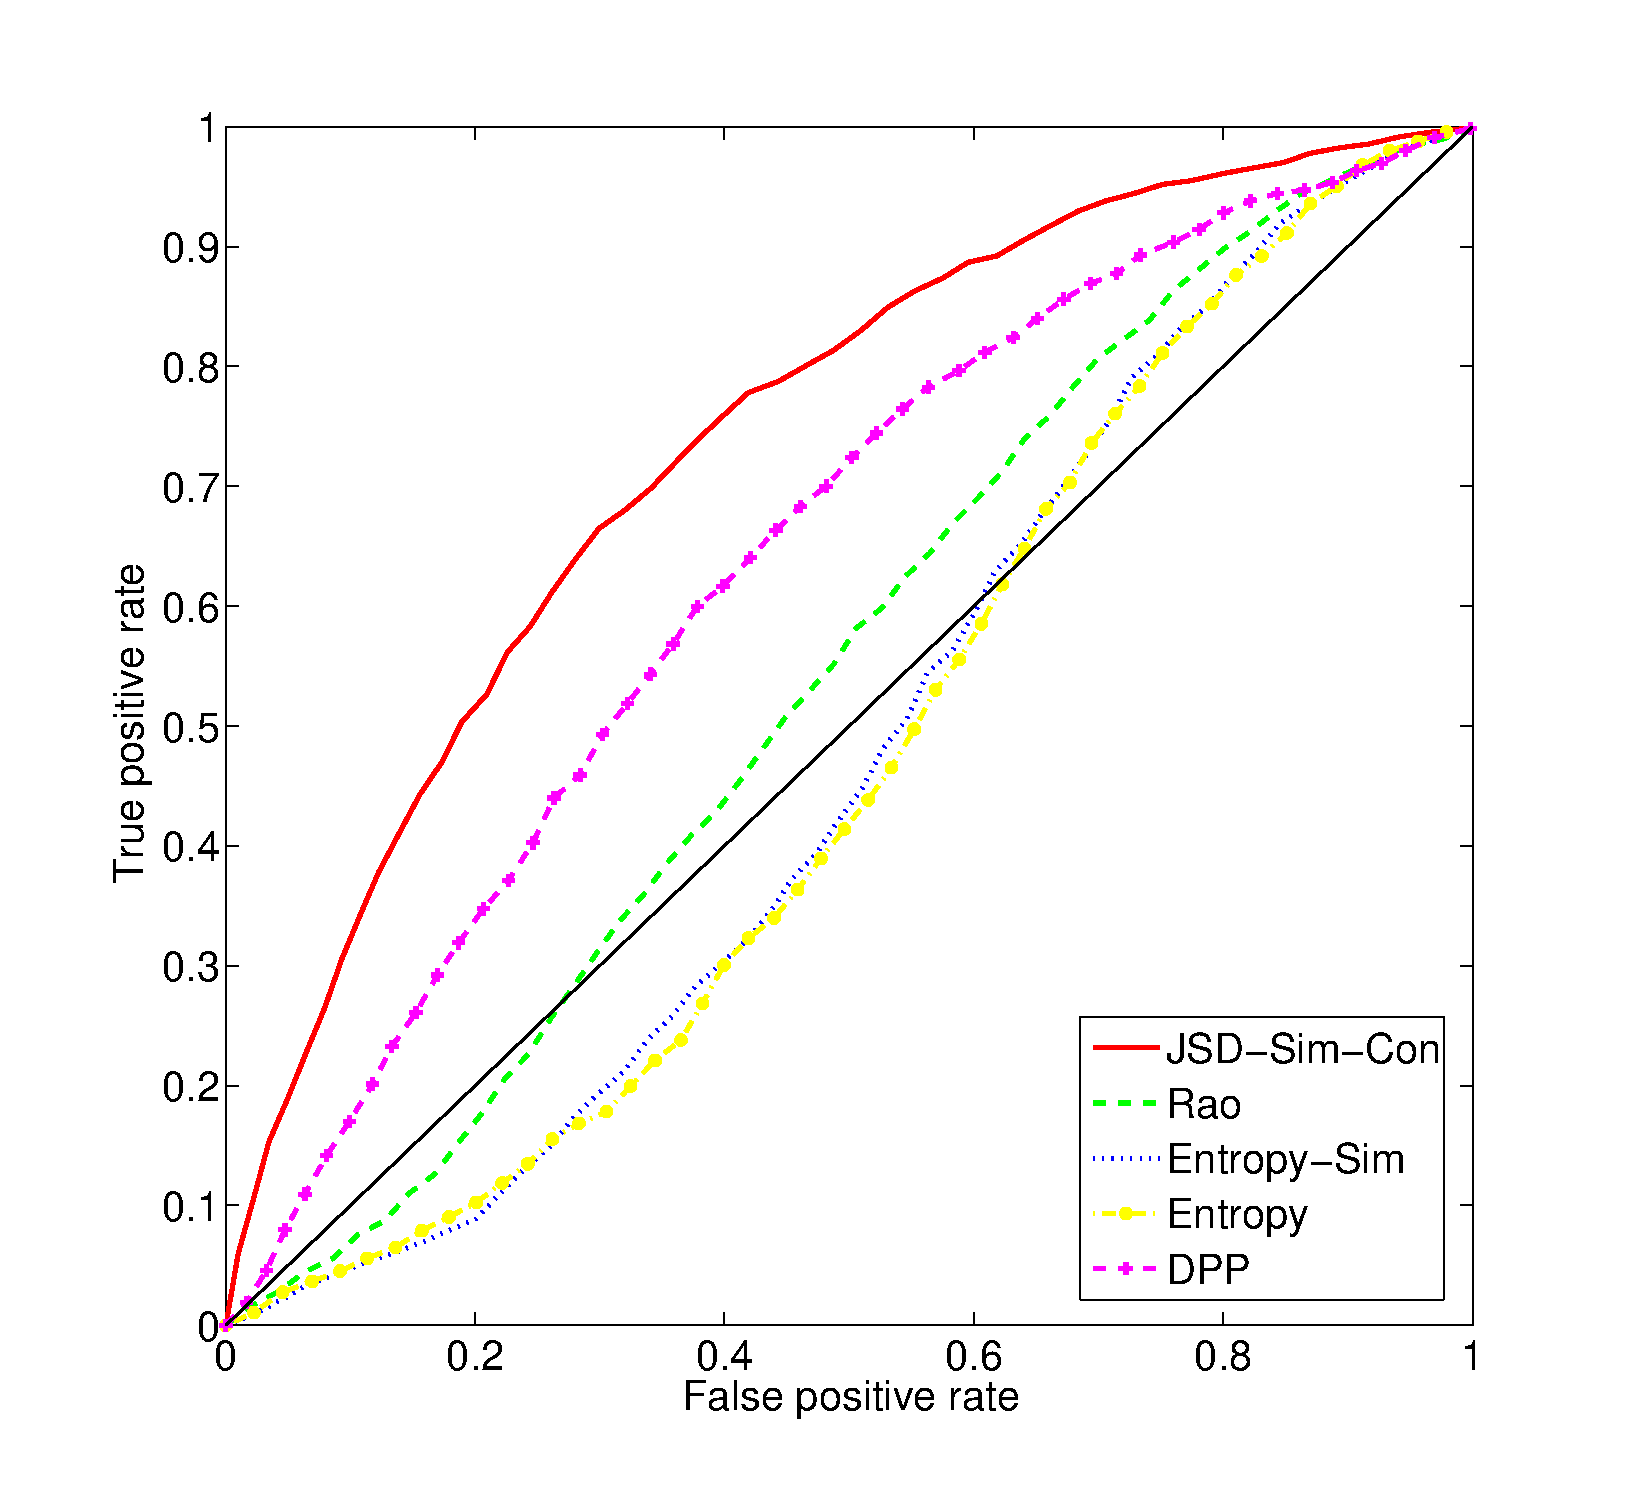
\includegraphics[width=0.45\textwidth]{figures/phonecases-comparison-new.eps}
    % \caption{}
\hspace{4mm}
  \end{subfigure}%
  ~
  \begin{subfigure}
(b) \hspace{-1mm}
    \centering
    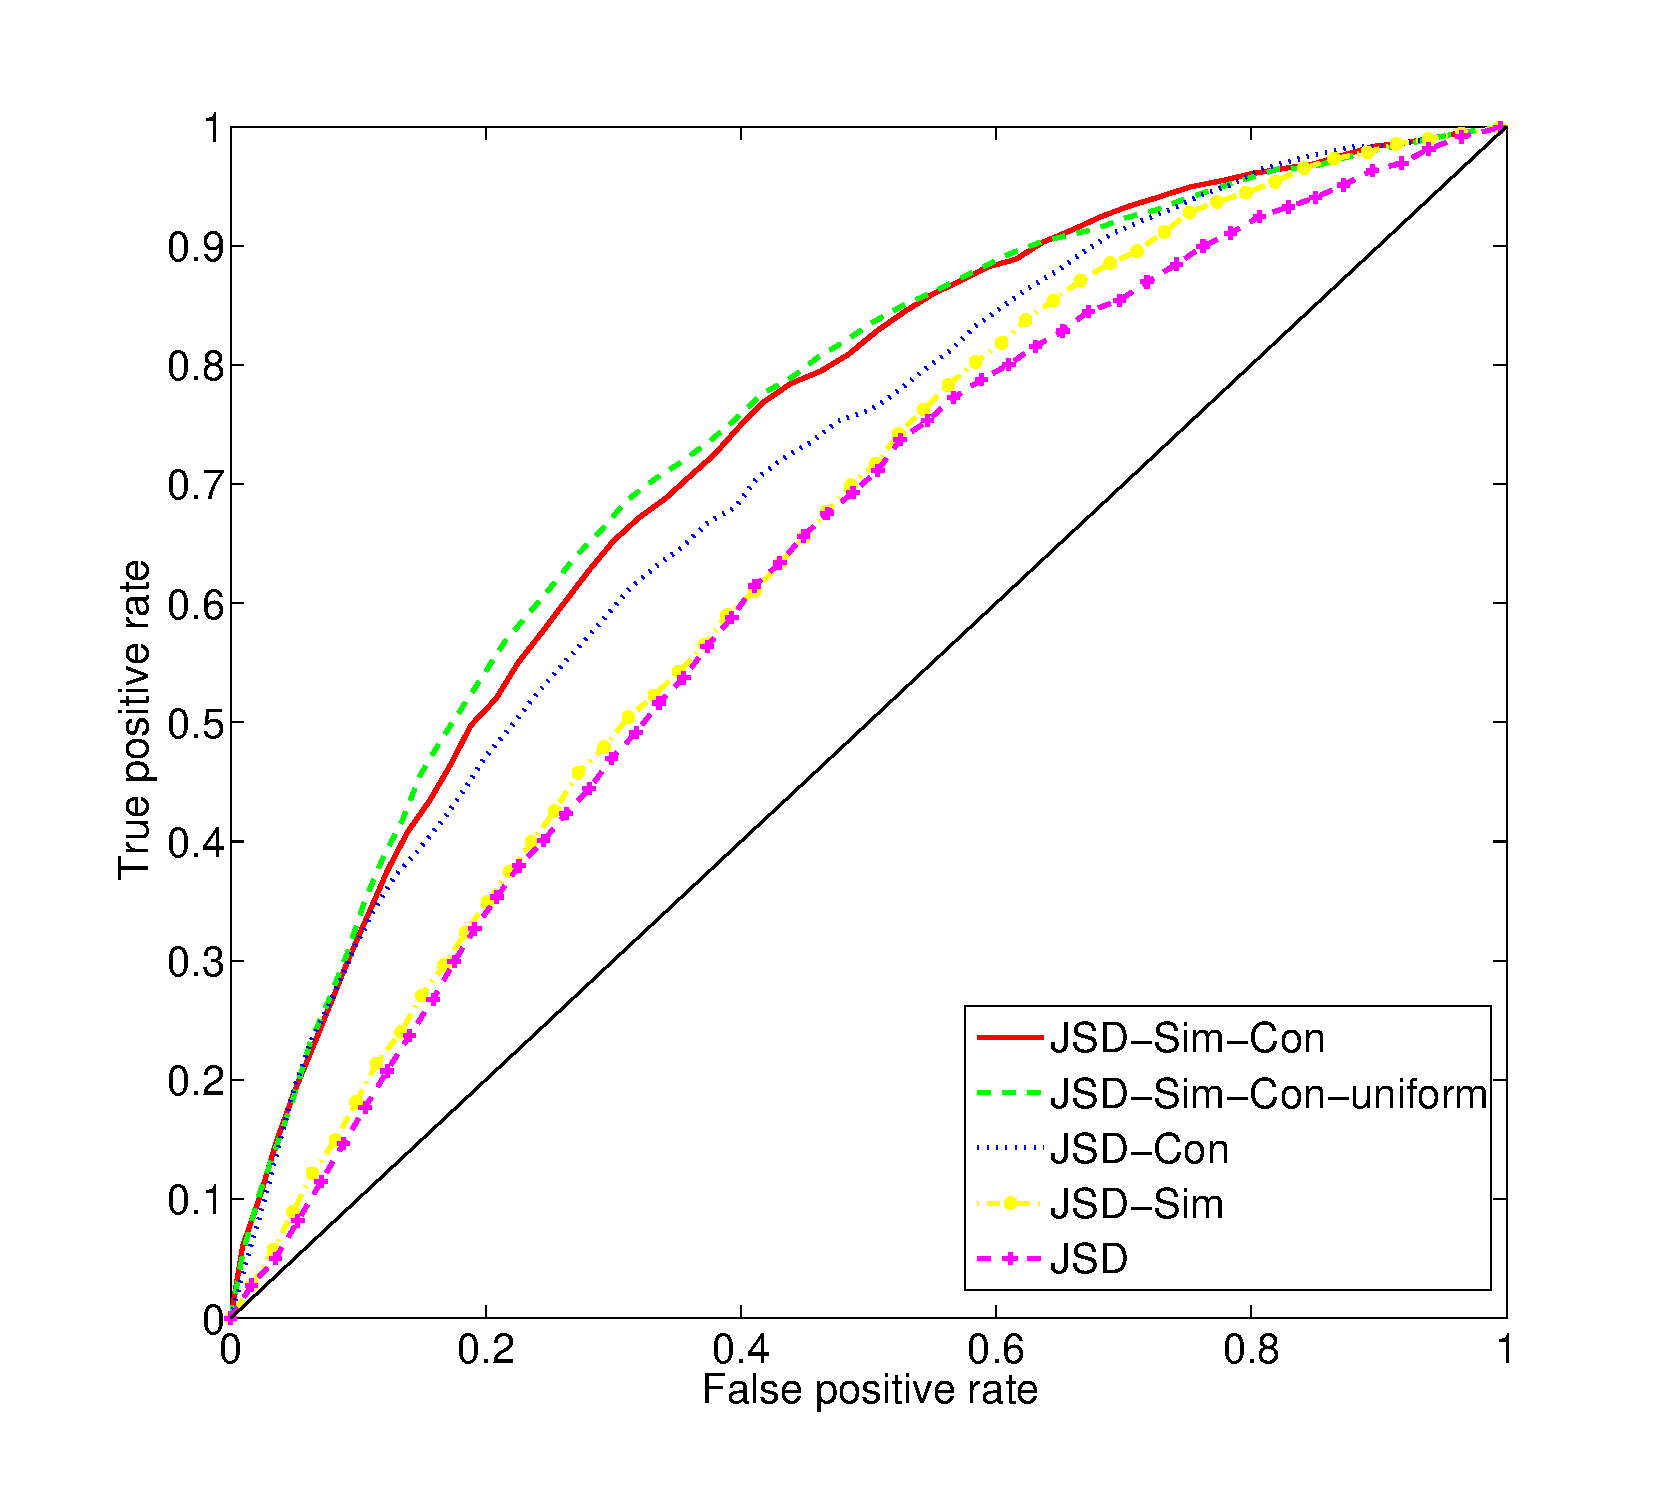
\includegraphics[width=0.45\textwidth]{figures/phonecases-breakdown-new.eps}
%    \caption{}
  \end{subfigure}
  
  \begin{subfigure}
(c) \hspace{-1mm}
    \centering
    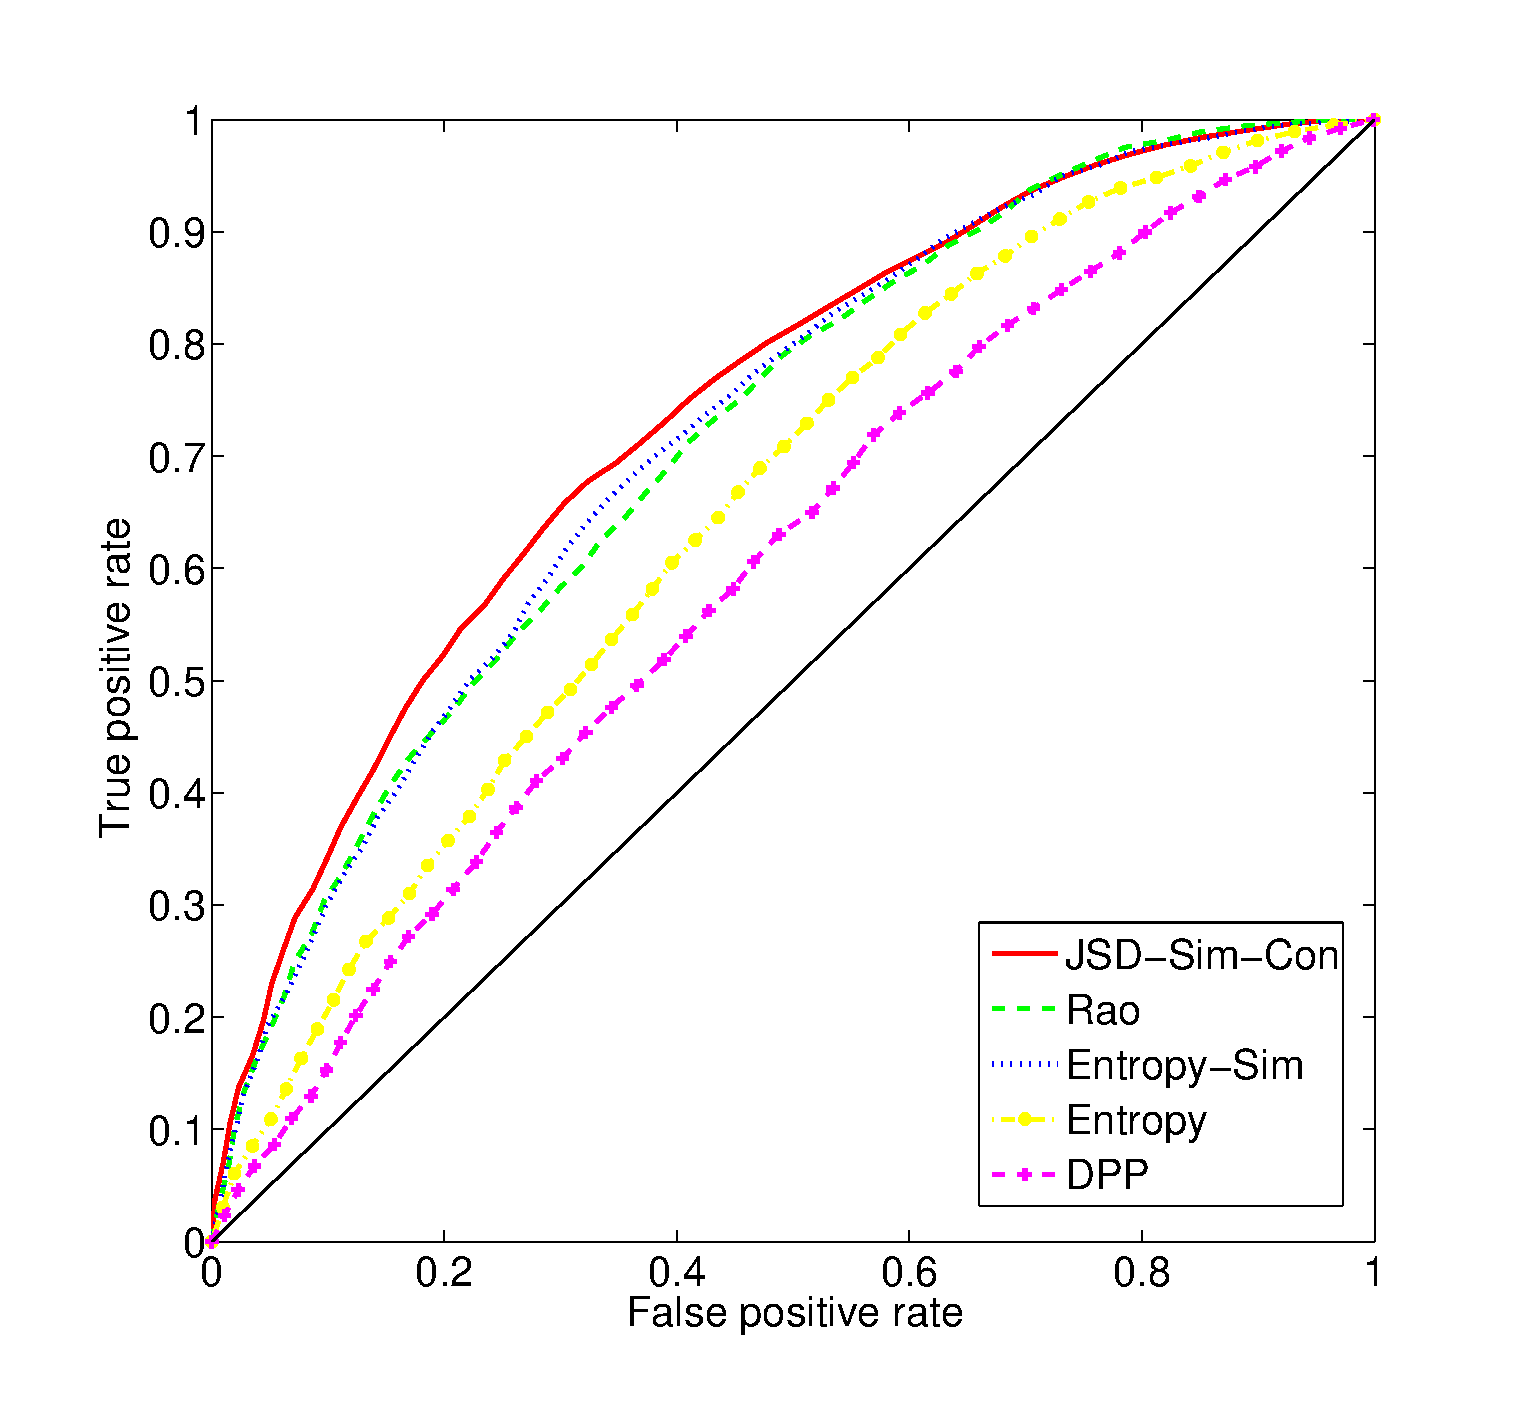
\includegraphics[width=0.45\textwidth]{figures/nsf-comparison-new.eps}
 %   \caption{}
\hspace{3mm}
  \end{subfigure}%
  ~
  \begin{subfigure}
(d) \hspace{-1mm}
    \centering
    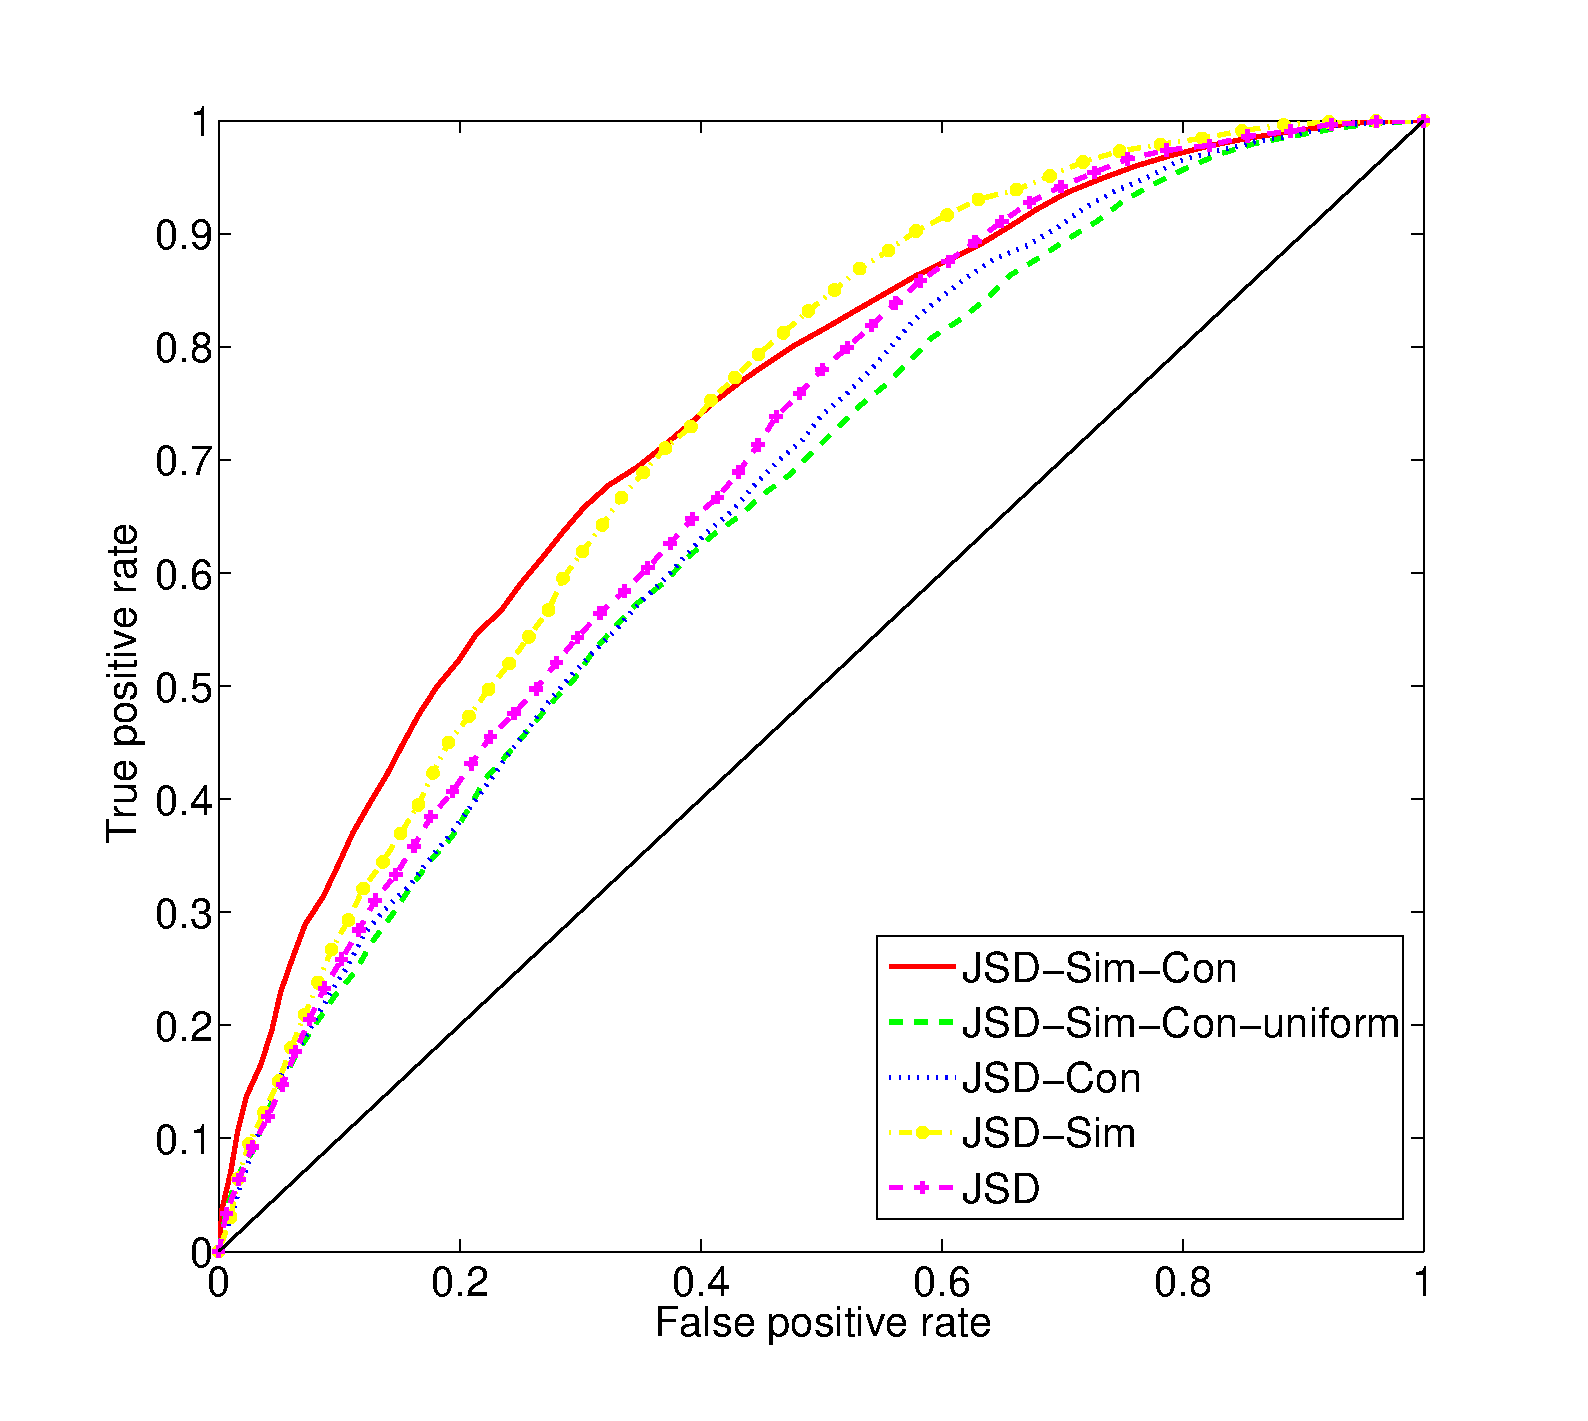
\includegraphics[width=0.45\textwidth]{figures/nsf-breakdown-new.eps}
 %   \caption{}
  \end{subfigure}

  \caption{ROC curves presenting the results of experiments on
 the eBay dataset (a,b) and NSF proposal dataset (c,d). The
 comparison plots (a,c) show the results for our approach (JSD-Sim-Con)
 against other methods, while the plots (b,d)
 show different variations of our approach. }
\label{fig:roc-curves}
\end{figure*}

%   \begin{table*}[t]
% \begin{center}
% \begin{tabular}{CC}
% 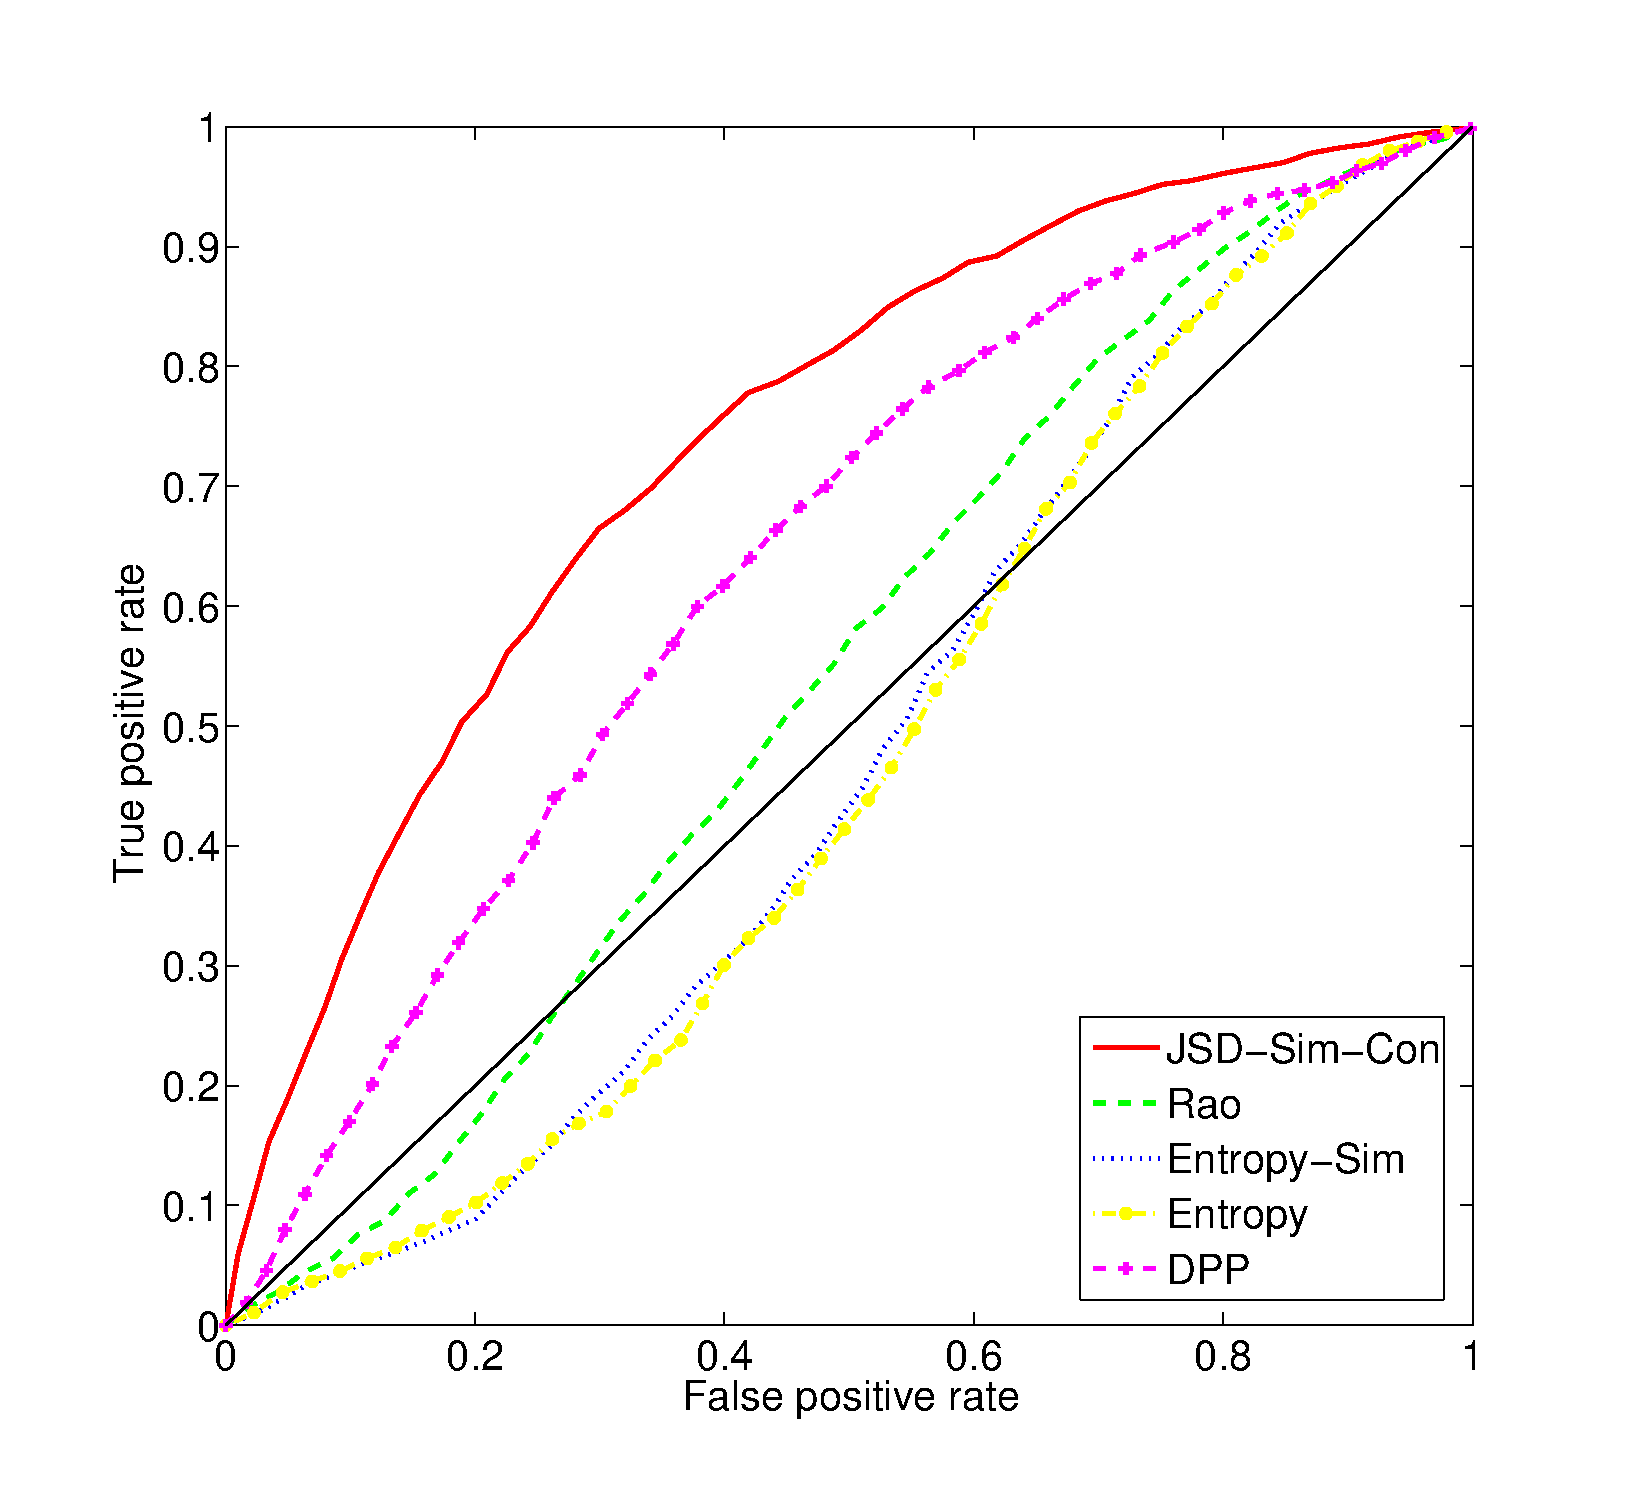
\includegraphics[height=6.5cm]{figures/phonecases-comparison-new.eps}&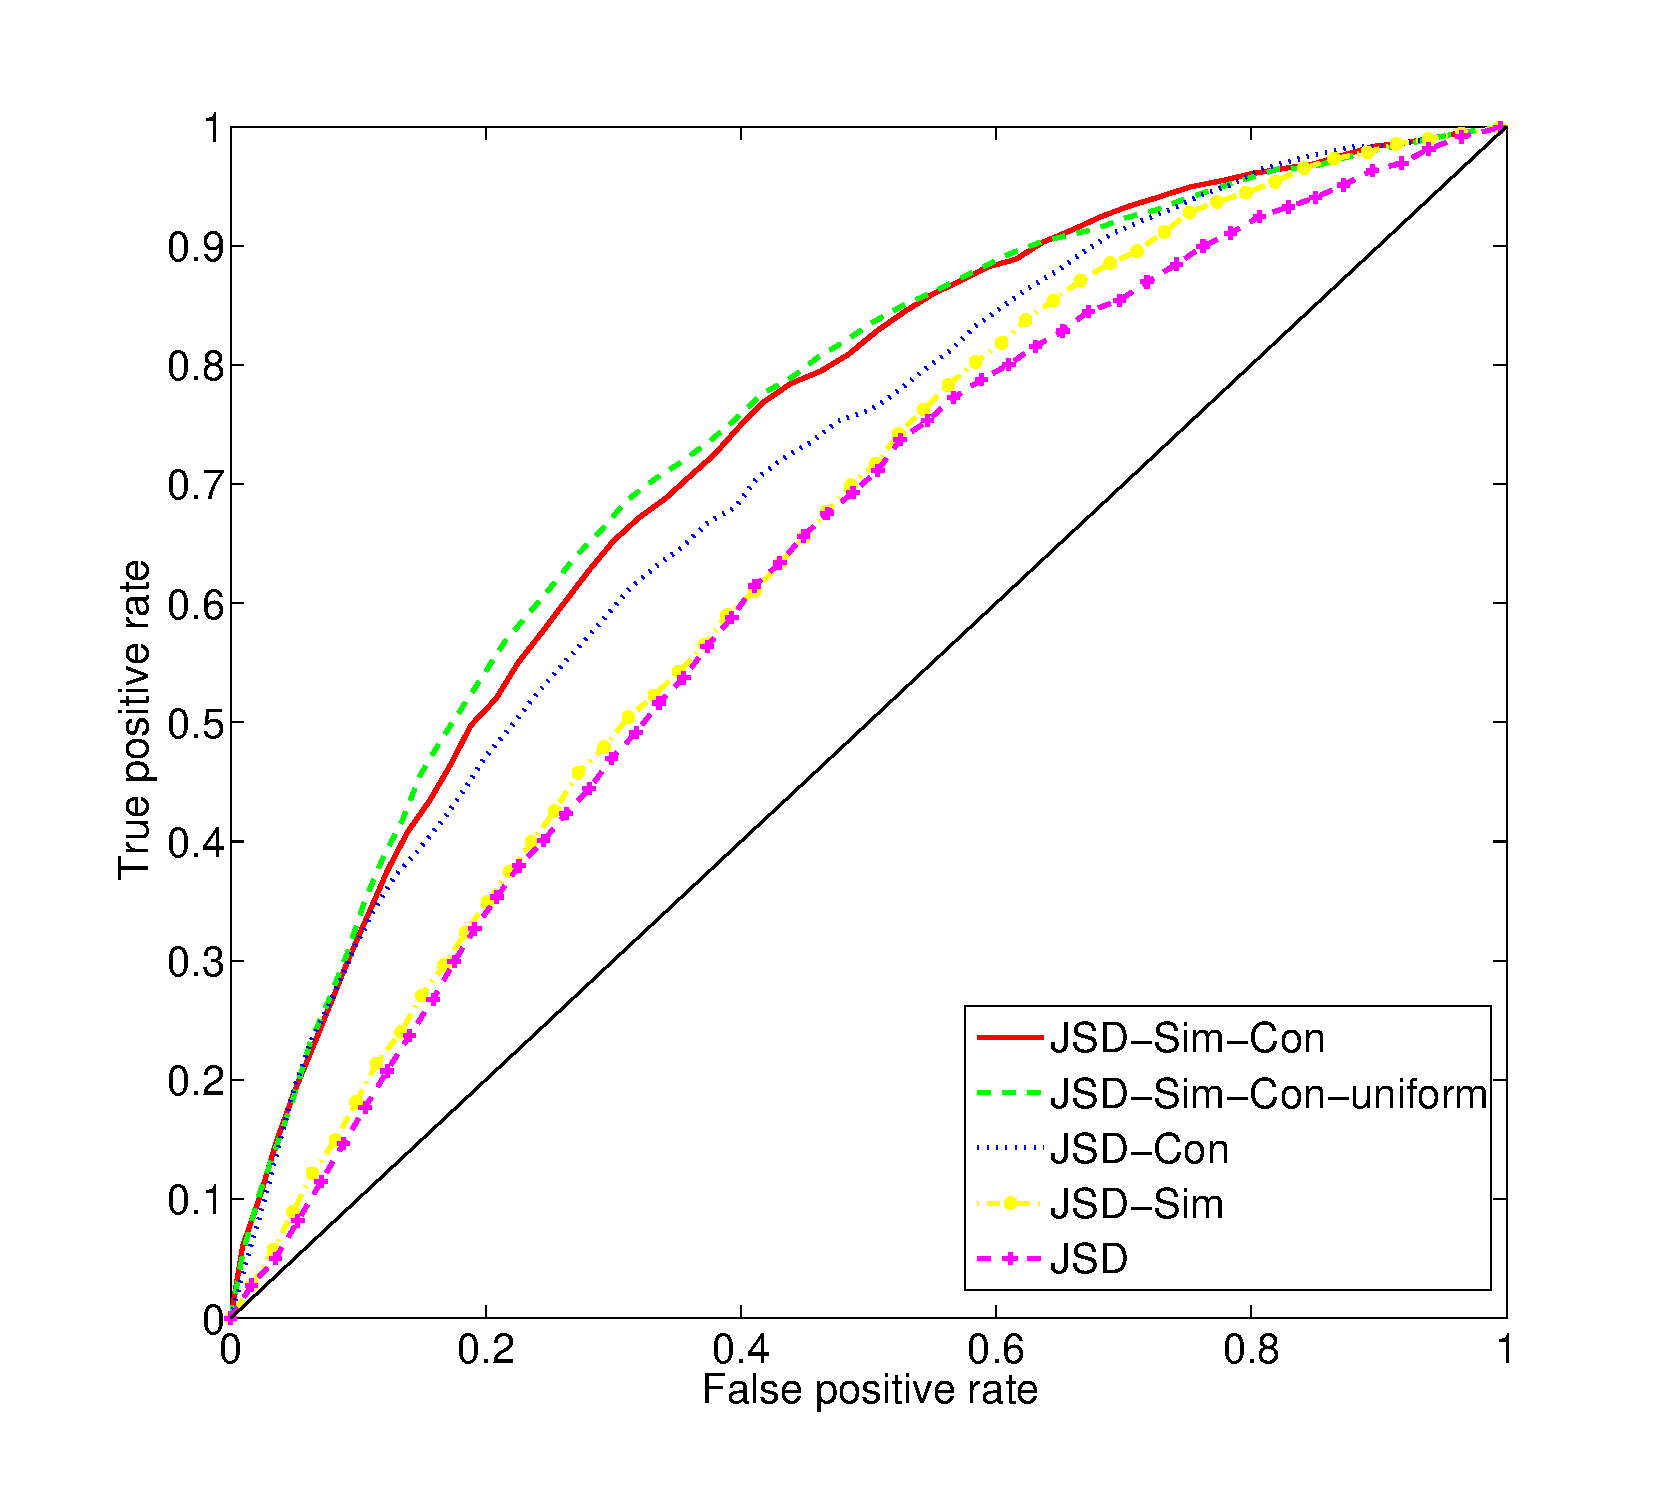
\includegraphics[height=6.5cm]{figures/phonecases-breakdown-new.eps}\\
% (a) & (b)\\
% 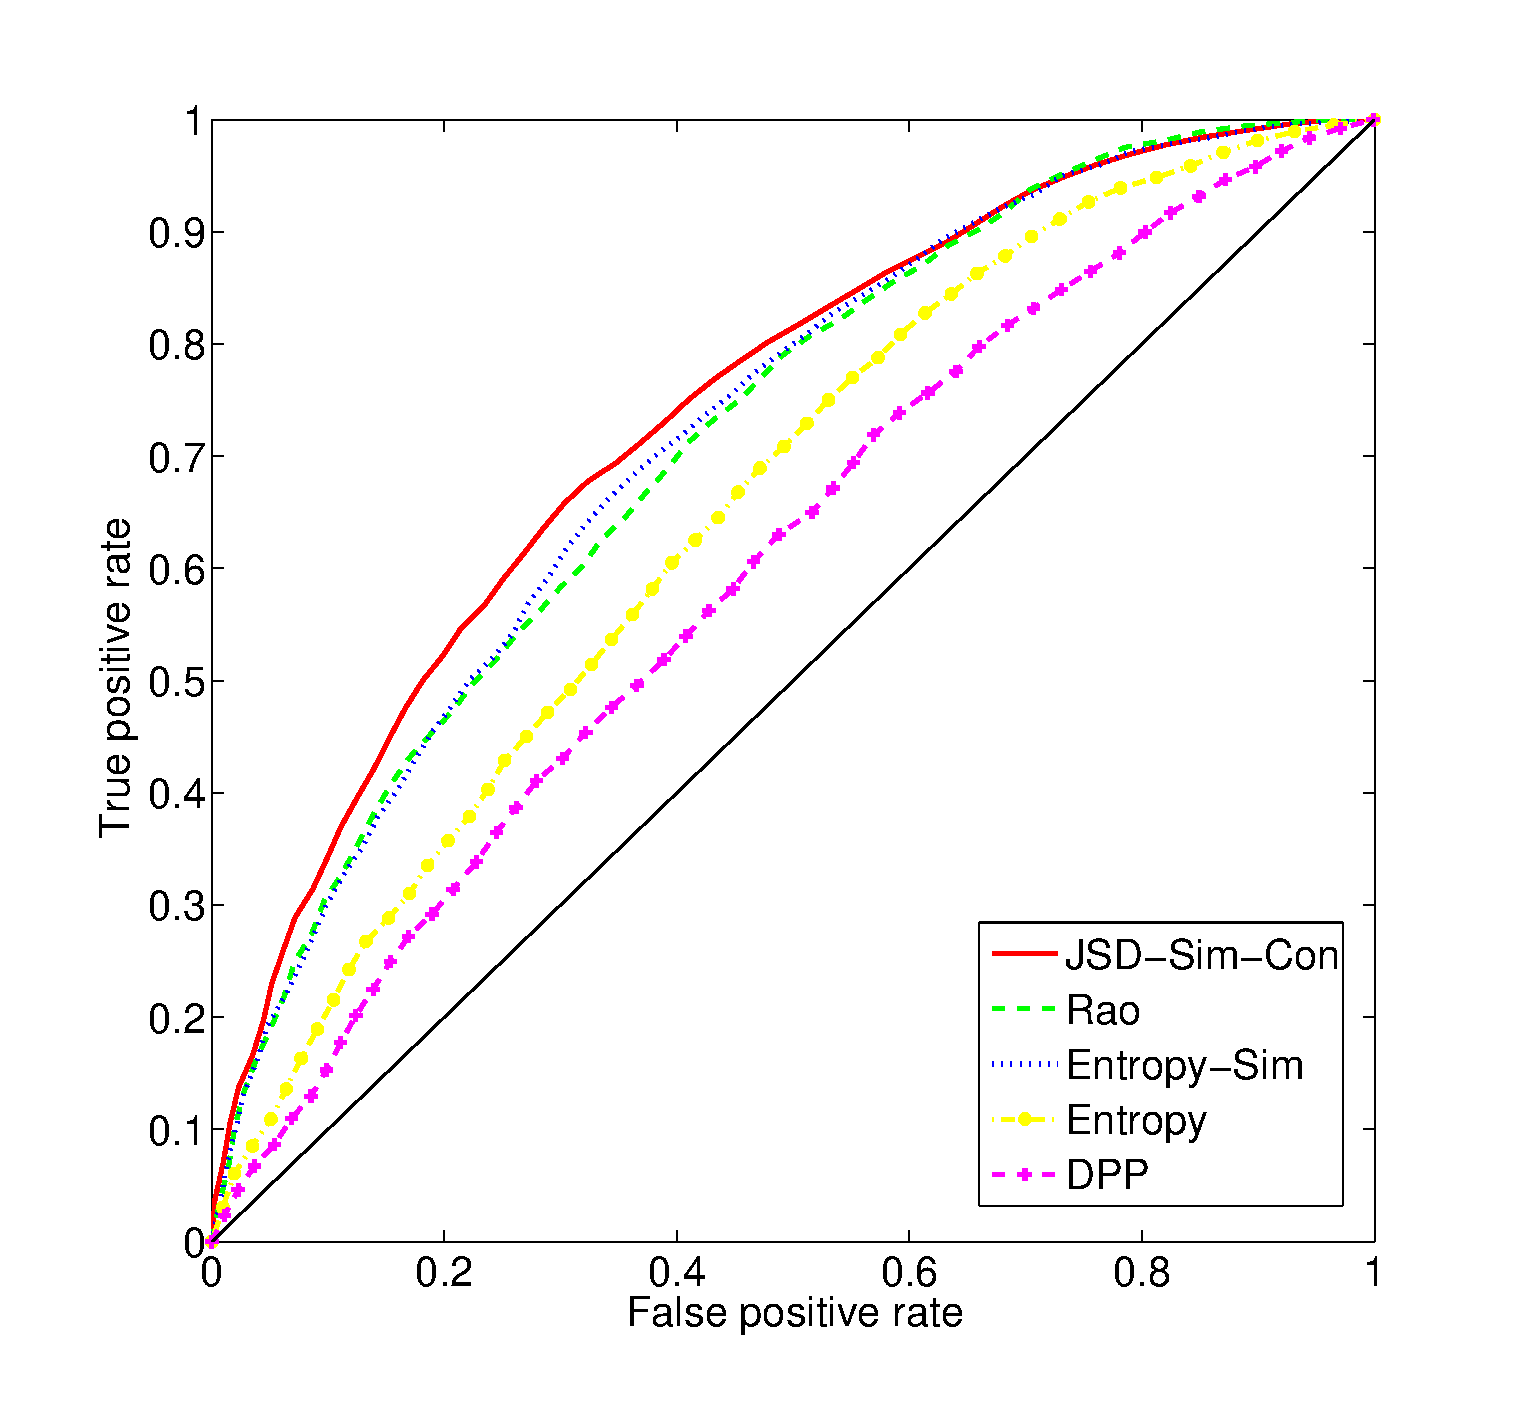
\includegraphics[height=6.5cm]{figures/nsf-comparison-new.eps}&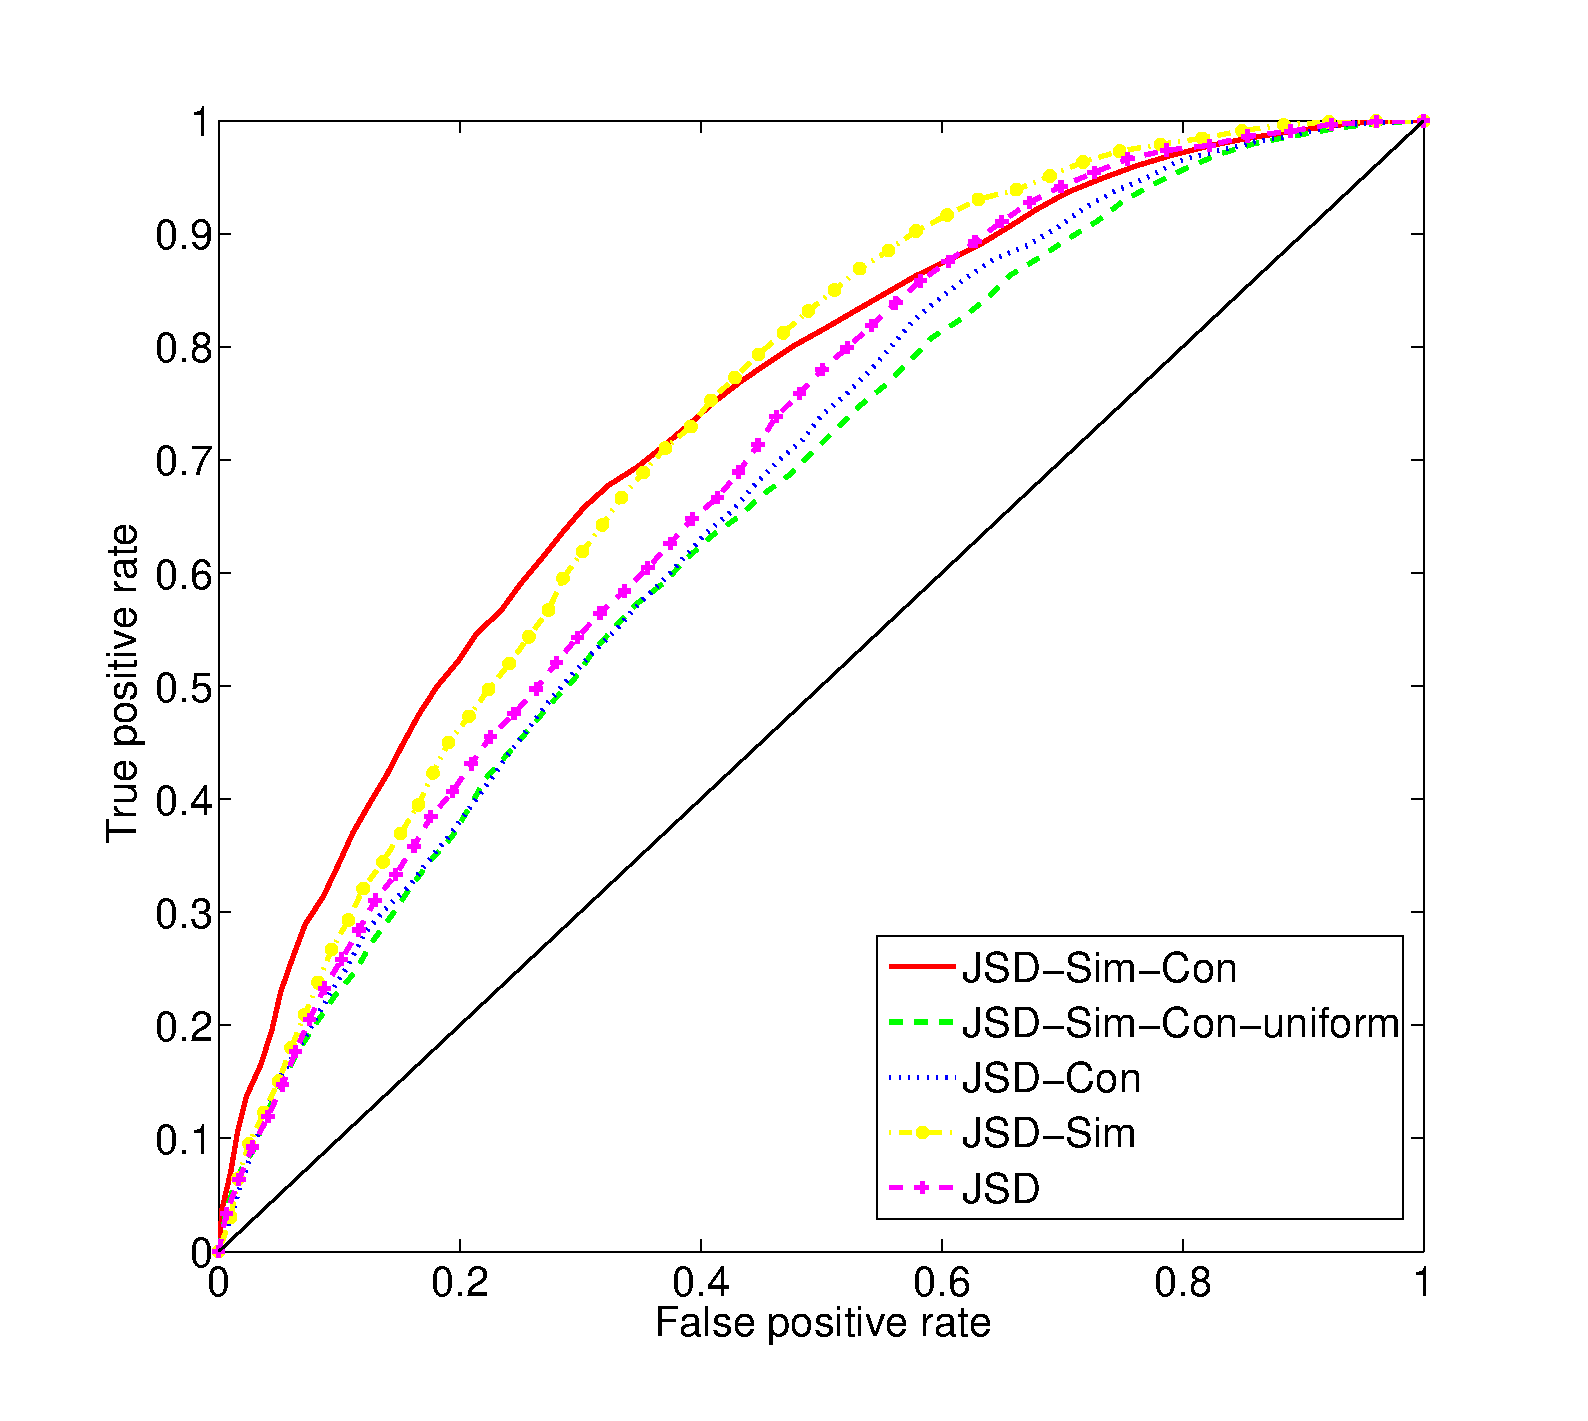
\includegraphics[height=6.5cm]{figures/nsf-breakdown-new.eps}\\
% (c) & (d)\\
% \end{tabular}
% \end{center}
% \caption{ROC curves presenting the results of experiments on
% the eBay dataset (a,b) and NSF proposal dataset (c,d). The
% comparison plots (a,c) show the results for our approach (JSD-Sim-Con)
% against other methods, while the plots (b,d)
% show different variations of our approach. }
% \label{fig:roc-curves}
% \end{table*}

